% !TeX program = xelatex
\documentclass{beamer}
% Metropolis theme for a modern look
\usetheme{metropolis}
% dopo \usetheme{…} e prima di \begin{document}
\setbeamercolor{background canvas}{bg=white}

\usefonttheme{professionalfonts}

% Encoding and language
\usepackage[utf8]{inputenc}
\usepackage[T1]{fontenc}
\usepackage[english]{babel}

% Graphics and math
\usepackage{graphicx}
\usepackage{booktabs}
\usepackage{amsmath}
\usepackage{xcolor}

% Metadata
\title{Aircraft Price Analysis}
\subtitle{Statistical Learning project}
\author{Amin Borqal, Filippo Bolis}
\date{\today}

\begin{document}

% Title page
\maketitle



% Section: Introduction and Key Questions
\section{Introduction and Key Questions}

\begin{frame}{Objective of the Analysis}
  Predict the price of aircraft using technical features and linear regression models with regularization.
\end{frame}

\begin{frame}{Key Questions About the Dataset}
  \begin{block}{}
    \begin{itemize}
      \item \textbf{qui mettiamo 2 domande che ci facciamo sul dataset }\\
            xxxxxxxxxxxdsvbiuwiofhwiohvioshiohvoiqervhoqeirhoeqrig.
      \item \textbf{Q: What is thegrsgjoiejgroiegjoqregtarget and in what units?}\\

    \end{itemize}
  \end{block}
\end{frame}

\begin{frame}{Dataset Description}
    \begin{itemize}
        \item \textbf{Total Observations}: 507
        \item \textbf{Total Variables}: 14
        \item \textbf{Numerical Variables}: 12
        \item \textbf{Categorical Variables}: 2
        \item \textbf{Target}: \texttt{price} (price in USD)
        \item \textbf{Source}: Kaggle – Aircraft Price Analysis \& Prediction Dataset
    \end{itemize}
\end{frame}

\begin{frame}{Numerical Variables 1}
    \begin{itemize}
        \item \texttt{engine\_power}: engine power (HP)
        \item \texttt{max\_speed}: maximum speed (km/h)
        \item \texttt{cruise\_speed}: cruise speed (km/h)
        \item \texttt{stall\_speed}: stall speed (km/h)
        \item \texttt{fuel\_tank}: fuel tank capacity (liters)
        \item \texttt{range}: range (km)
        \item \texttt{length}: aircraft length (m)
    \end{itemize}
\end{frame}

\begin{frame}{Numerical Variables 2}
    \begin{itemize}
        \item \texttt{wing\_span}: wingspan (m)
        \item \texttt{empty\_weight}: empty weight (kg)
        \item \texttt{all\_eng\_roc}: rate of climb with all engines (ft/min)
        \item \texttt{one\_eng\_roc}: rate of climb with one engine out (ft/min)
        \item \texttt{takeoff\_distance}: takeoff distance (m)
        \item \texttt{landing\_distance}: landing distance (m)
    \end{itemize}
\end{frame}

\begin{frame}{Categorical Variables}
    \begin{itemize}
        \item \texttt{model\_name}: aircraft model name
        \item \texttt{engine\_type}: type of engine
    \end{itemize}
\end{frame}

% Section: Data Preprocessing
\section{Data Preprocessing}
\begin{frame}{Data Cleaning}
  \begin{itemize}
    \item Removal of rows with missing values in the target \texttt{price}
    \item Checking and handling of outliers
    \item Necessary transformations to normalize distributions
  \end{itemize}
\end{frame}

\begin{frame}{Missing Data}
  \begin{itemize}
    \item 10 rows removed due to missing \texttt{price}
    \item Final dataset: 497 observations
  \end{itemize}
  \begin{center}
    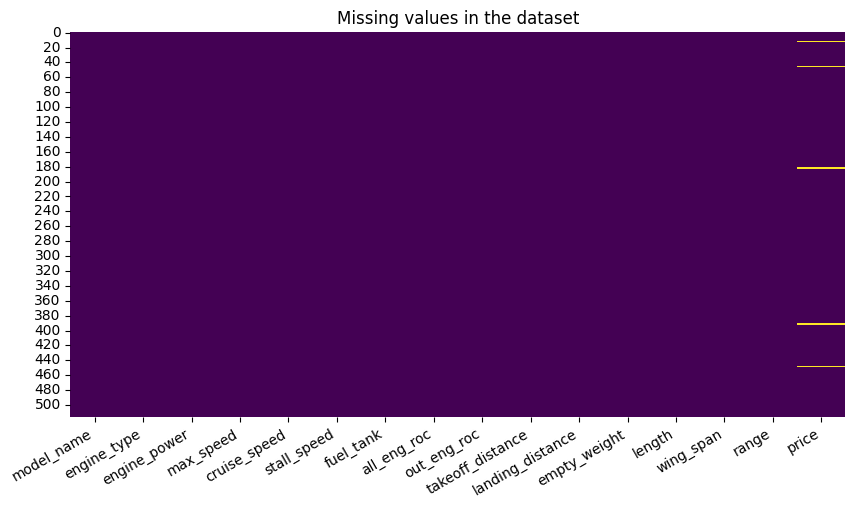
\includegraphics[width=1\linewidth]{images/missingValues.png}
  \end{center}
\end{frame}

\begin{frame}{Feature Distributions}
  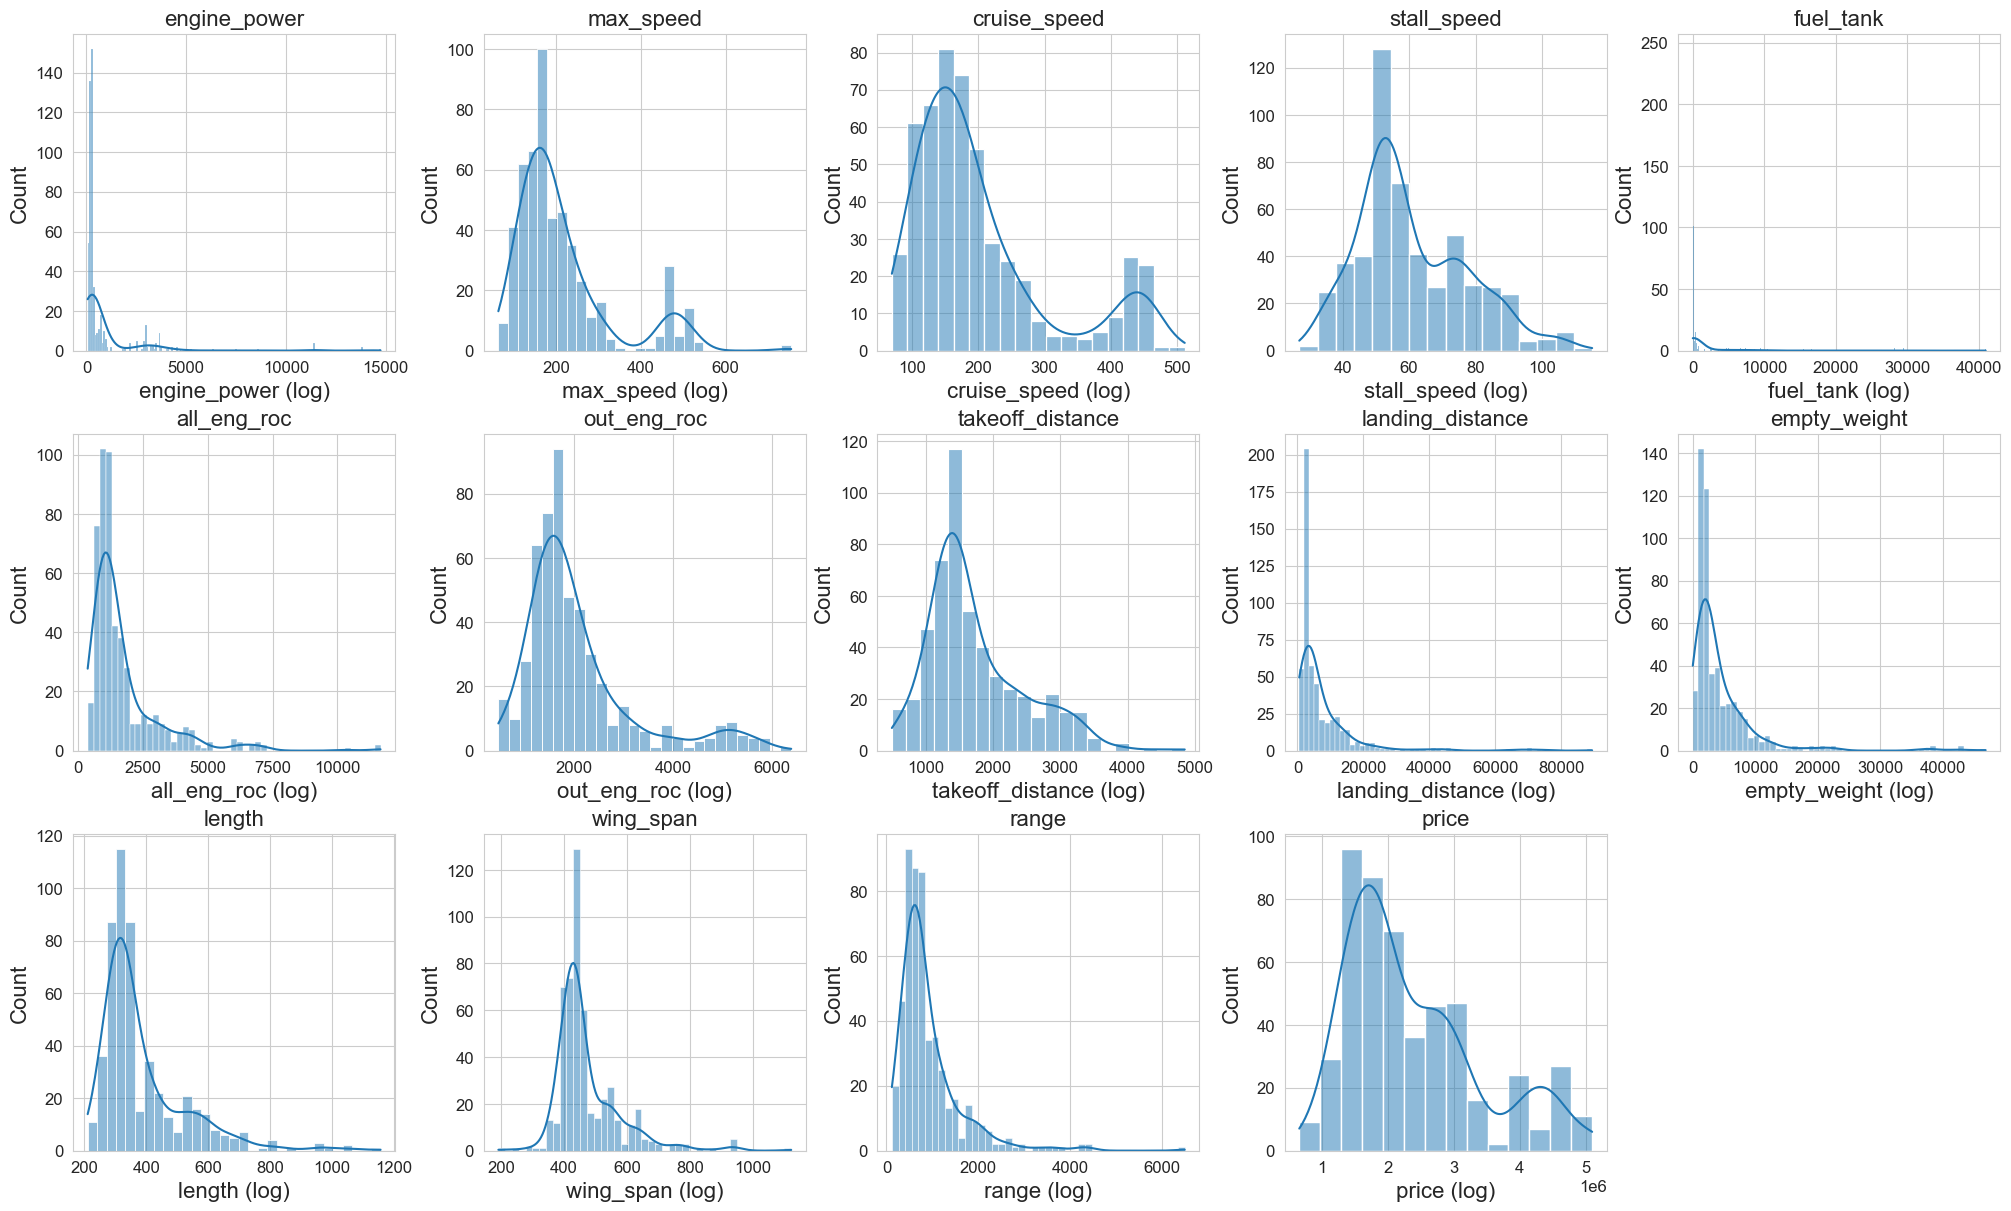
\includegraphics[width=1.01\linewidth]{images/FeaturesDistributions.png}
\end{frame}

\begin{frame}{Correlation Matrix}
  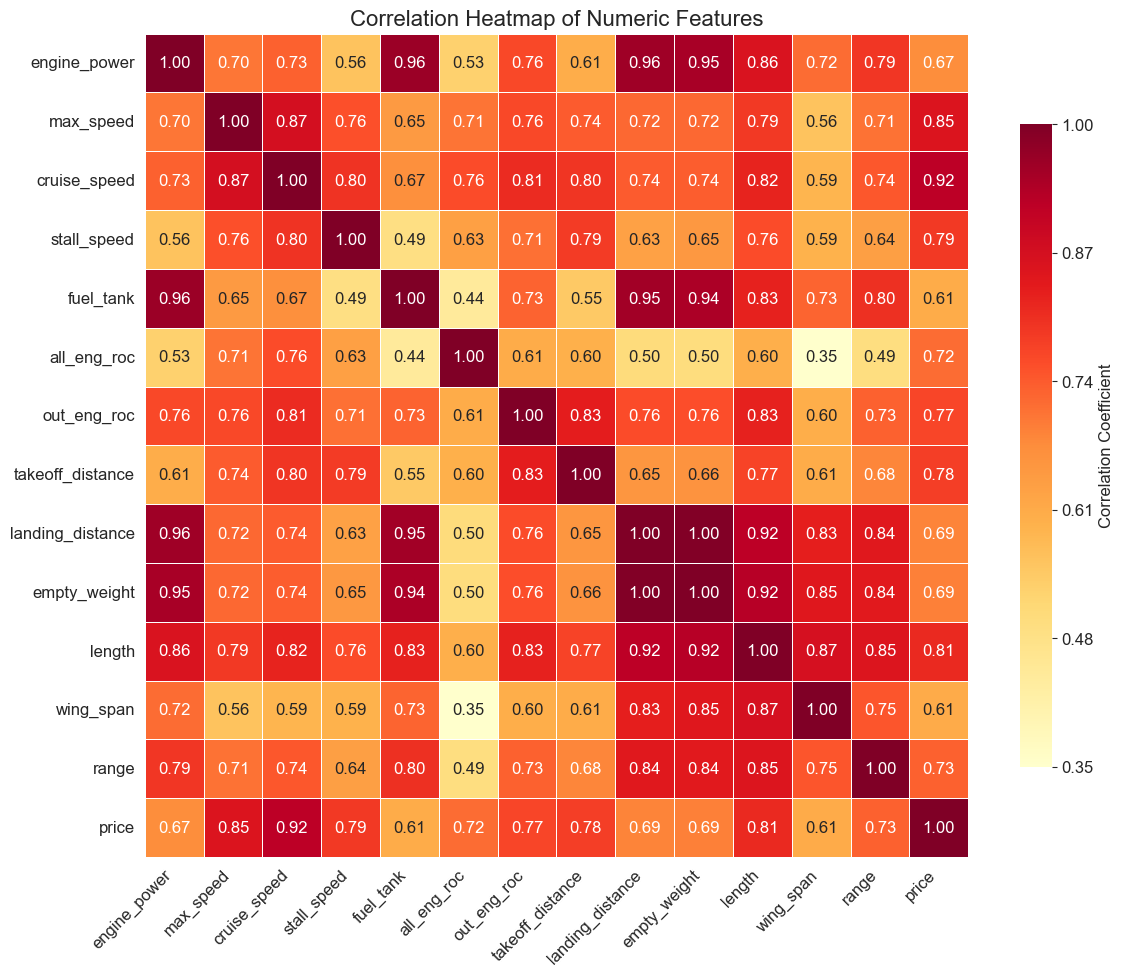
\includegraphics[width=0.9\linewidth]{images/Heatmap.png}
  \vspace{0.3cm}
  Evident multicollinearity among some variables, justifying the use of regularization.
\end{frame}

\begin{frame}{Dataset Comments}
  \begin{itemize}
    \item Numerical variables exhibit skewed distributions
    \item Correlations between variables suggest multicollinearity
    \item Transformations needed to improve linearity and normality
  \end{itemize}
\end{frame}

% Section: Log Transformation
\section{Log Transformation}
\begin{frame}{Motivations for Log Transformation}
    \begin{itemize}
        \item Numerical variables have \textbf{skewed} distributions
        \item Logarithmic transformation applied to all numerical features to:
        \begin{itemize}
            \item Achieve more symmetric distributions
            \item Improve linearity between features
            \item Reduce the impact of outliers
            \item Stabilize variance
        \end{itemize}
    \end{itemize}
\end{frame}

\begin{frame}{Distributions After Log Transformation}
    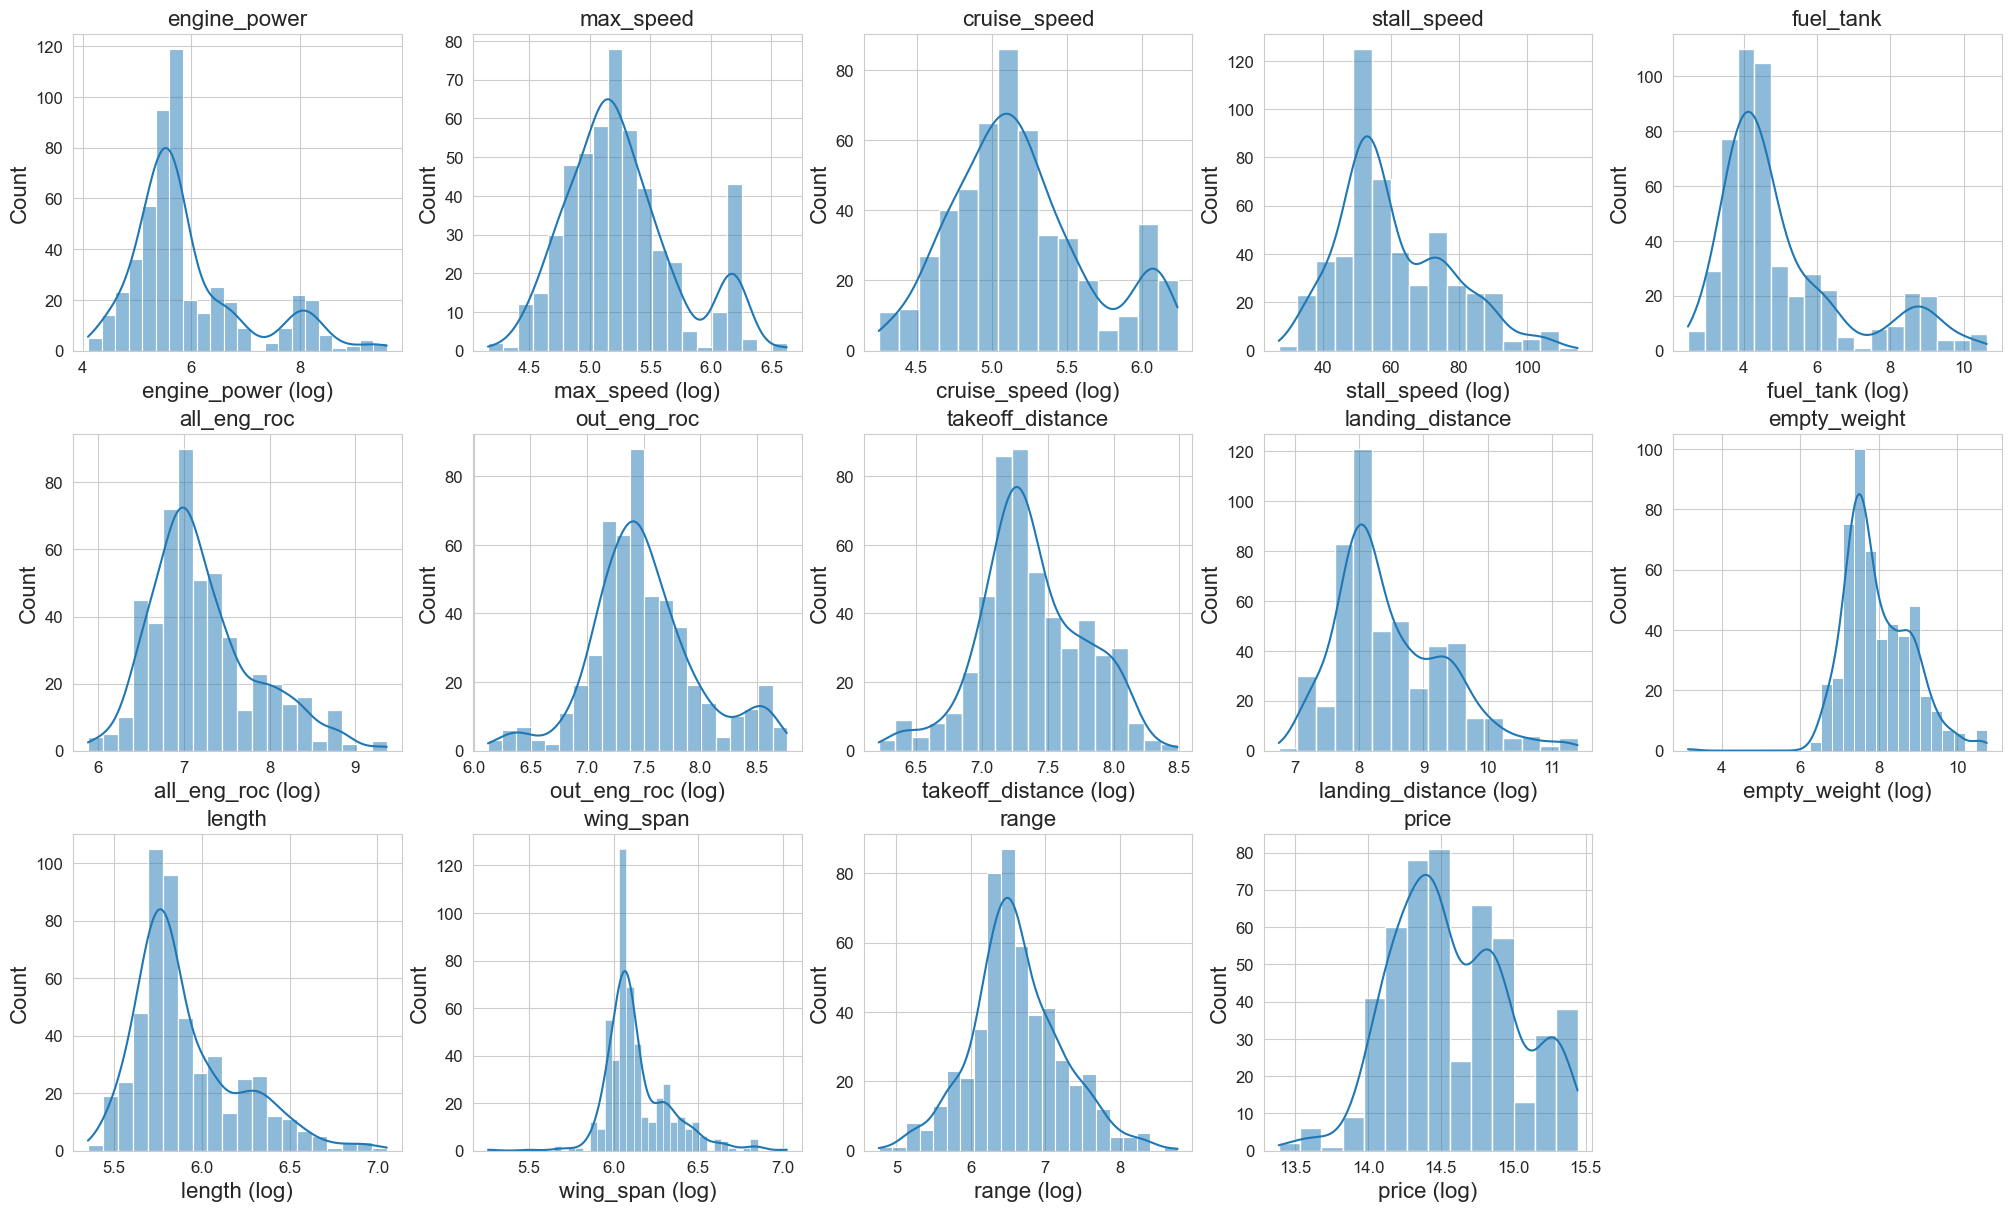
\includegraphics[width=1.01\linewidth]{images/Features-LOG-Distributions.png}
\end{frame}

\begin{frame}{Correlation Matrix After Log Transformation}
    \includegraphics[width=0.9\linewidth]{images/HeatmapLog.png}
    \vspace{0.3cm}
    Correlations changed after the logarithmic transformation.
\end{frame}

% Section: Linear Regression
\section{Linear Regression}
\subsection{Model with All Variables}
\begin{frame}{Multiple Linear Regression Model}
  \begin{equation*}
    \log(price) = \beta_0 + \sum_{j=1}^{13} \beta_j \log(x_j + 1) + \varepsilon
  \end{equation*}
  \begin{itemize}
    \item Preprocessing: log-transform of all numerical variables
    \item Validation: 10-fold CV with shuffling, \texttt{random\_state=42}
  \end{itemize}
\end{frame}

\begin{frame}[fragile]{K-Fold CV Metrics (Full)}
\begin{verbatim}
=== K-Fold CV Metrics ===
R^2 mean = 0.8282 ± 0.0585
MSE mean = 0.0275 ± 0.0080

RMSE (de-logged) = 391503.27 ± 0.0080
\end{verbatim}
\small{Inferential summary aggregated over the 10 training folds is shown in the next slide.}
\end{frame}

\begin{frame}{Inferential Summary (Full)}
\begin{tabular}{@{}lrrrr@{}}
    \toprule
    Feature          & coef$_{\text{mean}}$ & coef$_{\text{std}}$ & t$_{\text{mean}}$ & p$_{\text{mean}}$ \\
    \midrule
    engine\_power     & 0.011 & 0.021 &  0.37 & 0.543  \\
    max\_speed        & 0.175 & 0.026 &  4.64 & 0.001 \\
    cruise\_speed     & 0.504 & 0.039 &  9.73 & 0.001 \\
    stall\_speed      & 0.001 & 0.001 &  0.87 & 0.430  \\
    fuel\_tank        & 0.039 & 0.007 &  2.19 & 0.038  \\
    all\_eng\_roc      & 0.119 & 0.016 &  4.18 & 0.001 \\
    out\_eng\_roc      &-0.099 & 0.006 & -2.90 & 0.005  \\
    takeoff\_distance & 0.121 & 0.009 &  2.91 & 0.005  \\
    landing\_distance &-0.325 & 0.059 & -5.05 & 0.001 \\
    empty\_weight     & 0.104 & 0.050 &  2.66 & 0.008  \\
    length           & 0.155 & 0.046 &  1.48 & 0.178  \\
    wing\_span        & 0.367 & 0.078 &  3.88 & 0.001 \\
    range            & 0.025 & 0.011 &  1.06 & 0.336  \\
    \bottomrule
\end{tabular}
\end{frame}

\subsection{Model with Only Significant Variables}
\begin{frame}{Reduced Model (Only Significant Variables)}
    \begin{itemize}
        \item Selected the 9 features with \(p < 0.05\)
        \item \textbf{Removed Features}: engine\_power, stall\_speed, length, range
        \item Retrained with the same CV settings
    \end{itemize}
\end{frame}

\begin{frame}{Reduced Model vs Full Model Results}
    \begin{block}{}
        \begin{columns}
            \begin{column}{0.48\textwidth}
                \centering
                \textbf{Full Model}\\
                \textcolor{gray}{\small(14 features)}
                \vspace{0.3cm}
                \begin{tabular}{@{}ll@{}}
                    R² mean & 0.8282 ± 0.0585 \\
                    MSE mean & 0.0275 ± 0.0080 \\
                    RMSE (USD) & \$391{,}503.27 \\
                \end{tabular}
            \end{column}
            \begin{column}{0.48\textwidth}
                \centering
                \textbf{Reduced Model}\\
                \textcolor{gray}{\small(9 features)}
                \vspace{0.3cm}
                \begin{tabular}{@{}ll@{}}
                    R² mean & 0.8291 ± 0.0643 \\
                    MSE mean & 0.0271 ± 0.0080 \\
                    RMSE (USD) & \$389{,}179.25 \\
                \end{tabular}
            \end{column}
        \end{columns}
    \end{block}
    
    \vspace{0.5cm}
    \begin{block}{}
        \begin{itemize}
            \item \textbf{Slight improvement} in R² and RMSE
        \end{itemize}
    \end{block}
\end{frame}

\begin{frame}{Coefficients of Reduced Model}
  \begin{tabular}{@{}lrrrrr@{}}
    \toprule
    Feature          & coef$_{\text{mean}}$ & coef$_{\text{std}}$ & t$_{\text{mean}}$ & p$_{\text{mean}}$ \\
    \midrule
    intercept        & 8.515 & 0.311 & 16.37 & 0.001 \\
    max\_speed        & 0.179 & 0.024 &  4.84 & 0.001 \\
    cruise\_speed     & 0.522 & 0.032 & 10.81 & 0.001 \\
    fuel\_tank        & 0.049 & 0.005 &  3.60 & 0.001 \\
    all\_eng\_roc      & 0.125 & 0.014 &  4.50 & 0.001 \\
    out\_eng\_roc      &-0.084 & 0.007 & -2.57 & 0.013  \\
    takeoff\_distance & 0.132 & 0.006 &  3.44 & 0.001 \\
    landing\_distance &-0.285 & 0.059 & -5.43 & 0.001 \\
    empty\_weight     & 0.109 & 0.057 &  2.82 & 0.006  \\
    wing\_span        & 0.405 & 0.057 &  4.75 & 0.001 \\
    \bottomrule
  \end{tabular}
\end{frame}

\subsection{Residual Analysis}
\begin{frame}{Residual Analysis}
      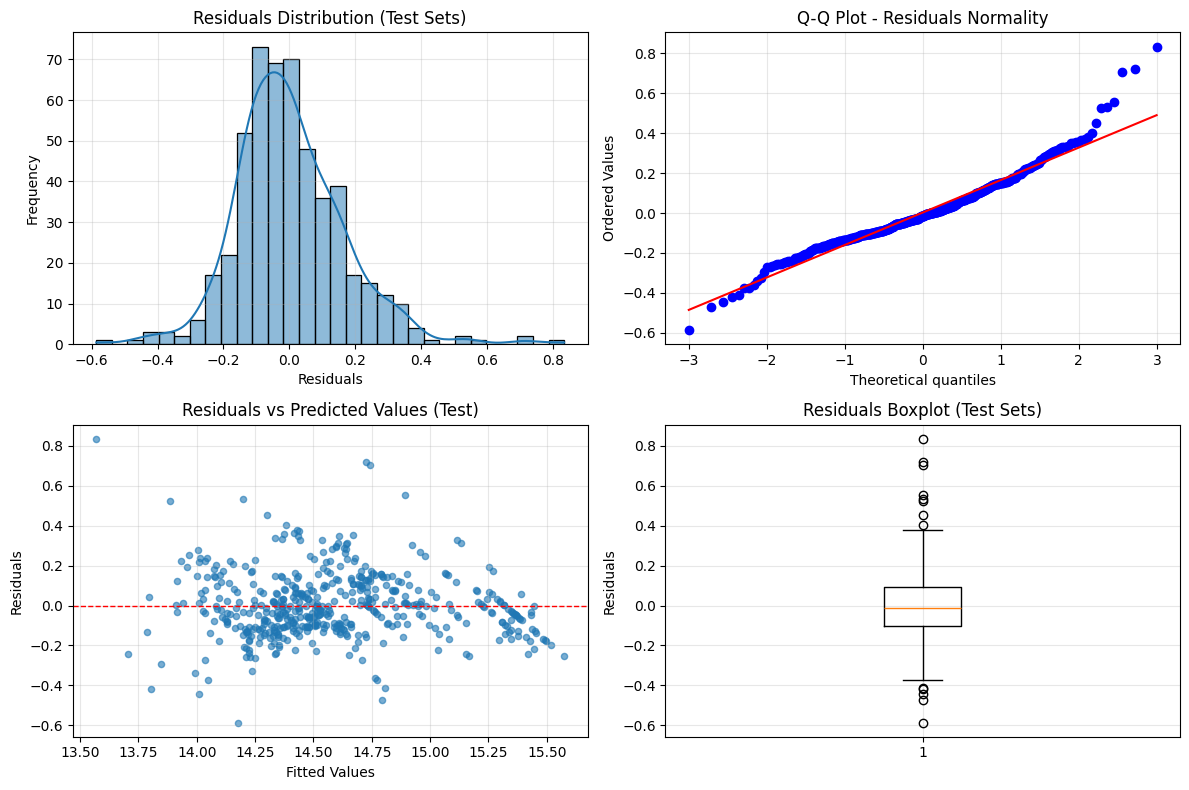
\includegraphics[width=\linewidth]{images/RegressionResidualsCV.png}
\end{frame}
\begin{frame}{Residual Analysis: Observations}
    \begin{itemize}
        \item Residuals exhibit a symmetric distribution
        \item No obvious patterns, suggesting the model captures the variable relationships well
        \item A few observations have larger residuals, but no extreme outliers
    \end{itemize}
\end{frame}

% Section: Regularization
\section{Regularization}

\subsection{Ridge}
\begin{frame}{Ridge Regression}
    \begin{equation*}
        \min_{\beta} \left\{ \frac{1}{2n} \lVert y - X\beta\rVert_2^2 + \alpha \lVert \beta \rVert_2^2 \right\}
    \end{equation*}
    \begin{itemize}
        \item L2 penalty on coefficients
        \item Uses all features
        \item Cross-validation to select the best $\alpha$
        \item Objective: reduce overfitting and improve generalization
    \end{itemize}
\end{frame}

\begin{frame}{Ridge: Metrics and Coefficients}
        \begin{columns}
                \begin{column}{0.48\textwidth}
                        \centering
                        \textbf{Best $\alpha$ and Metrics}
                        \vspace{0.3cm}
                        \begin{tabular}{@{}lc@{}}
                                \toprule
                                \textbf{Parameter} & \textbf{Value} \\
                                \midrule
                                Best $\alpha$        & 13.2070 \\
                                Test MSE             & 0.0249 \\
                                Test RMSE            & 0.1579 \\
                                Test MAE             & 0.1182 \\
                                Test R$^2$           & 0.8584 \\
                                \bottomrule
                        \end{tabular}
                \end{column}
                \begin{column}{0.68\textwidth}
                        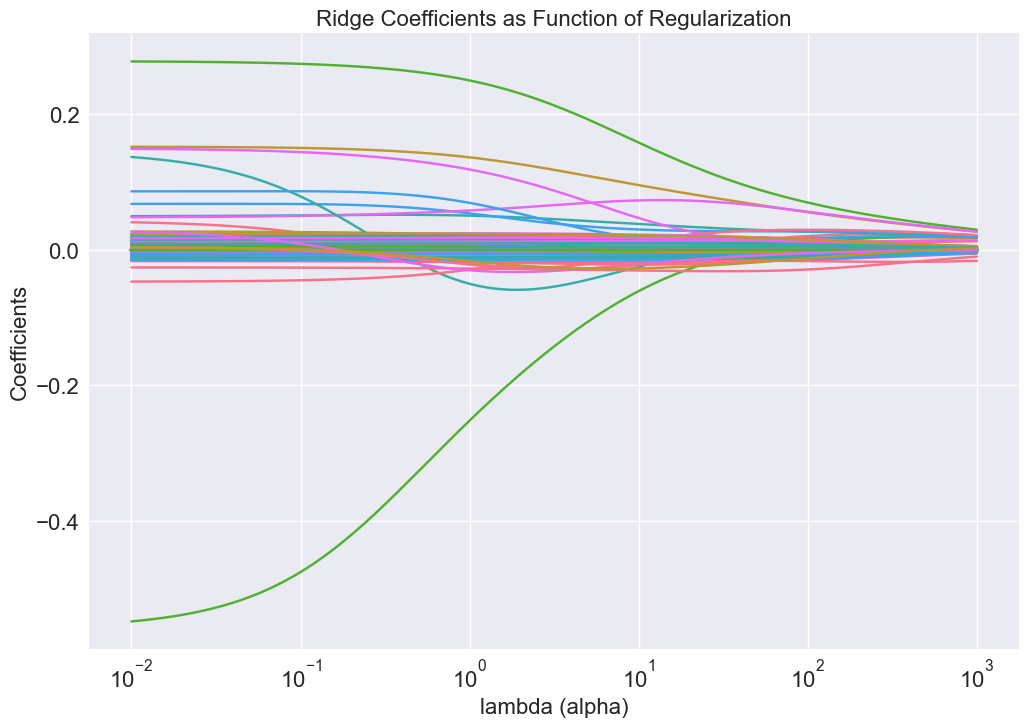
\includegraphics[width=\linewidth]{images/Ridge.png}
                        \vspace{0.1cm}
                        \small{Ridge coefficients after regularization.}
                \end{column}
        \end{columns}
\end{frame}

\begin{frame}{Ridge: Cross-Validation Error}
        \begin{center}
                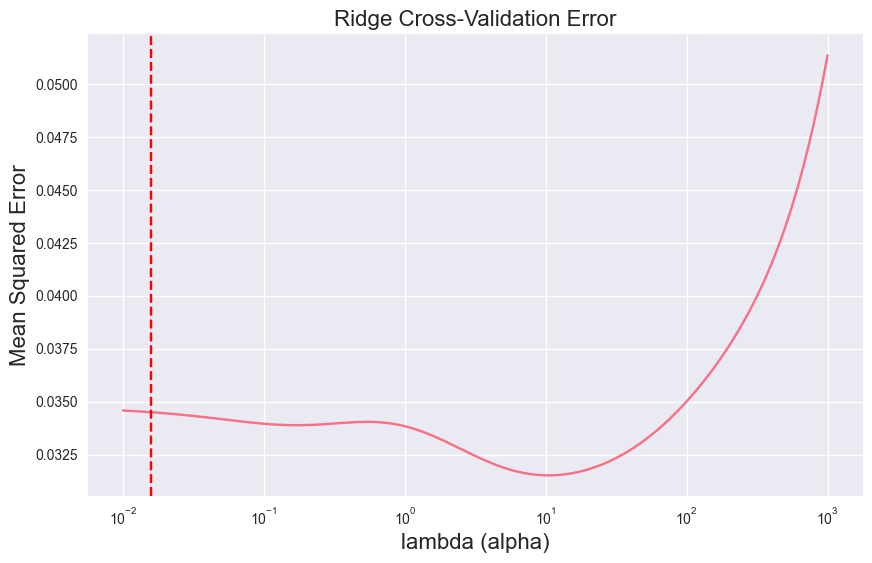
\includegraphics[width=0.9\linewidth]{images/RidgeCV.png}
        \end{center}
        Cross-validation error as a function of $\alpha$ for selecting the optimal parameter.
\end{frame}

\subsection{Lasso}
\begin{frame}{Lasso Regression}
    \begin{equation*}
        \min_{\beta} \left\{ \frac{1}{2n} \lVert y - X\beta\rVert_2^2 + \alpha \lVert \beta \rVert_1 \right\}
    \end{equation*}
    \begin{itemize}
        \item L1 penalty: automatic feature selection
        \item Coefficients can be driven to zero
        \item Cross-validation to select the best $\alpha$
        \item Objective: interpretability and dimensionality reduction
    \end{itemize}
\end{frame}

\begin{frame}{Lasso: Metrics and Coefficients}
        \begin{columns}
                \begin{column}{0.48\textwidth}
                        \centering
                        \textbf{Best $\alpha$ and Metrics}
                        \vspace{0.3cm}
                        \begin{tabular}{@{}lc@{}}
                                \toprule
                                \textbf{Parameter} & \textbf{Value} \\
                                \midrule
                                Best $\alpha$        & 0.0159 \\
                                Test MSE             & 0.0257 \\
                                Test RMSE            & 0.1604 \\
                                Test MAE             & 0.1192 \\
                                Test R$^2$           & 0.8539 \\
                                Selected Features    & 16 / 290 \\
                                \bottomrule
                        \end{tabular}
                \end{column}
                \begin{column}{0.68\textwidth}
                        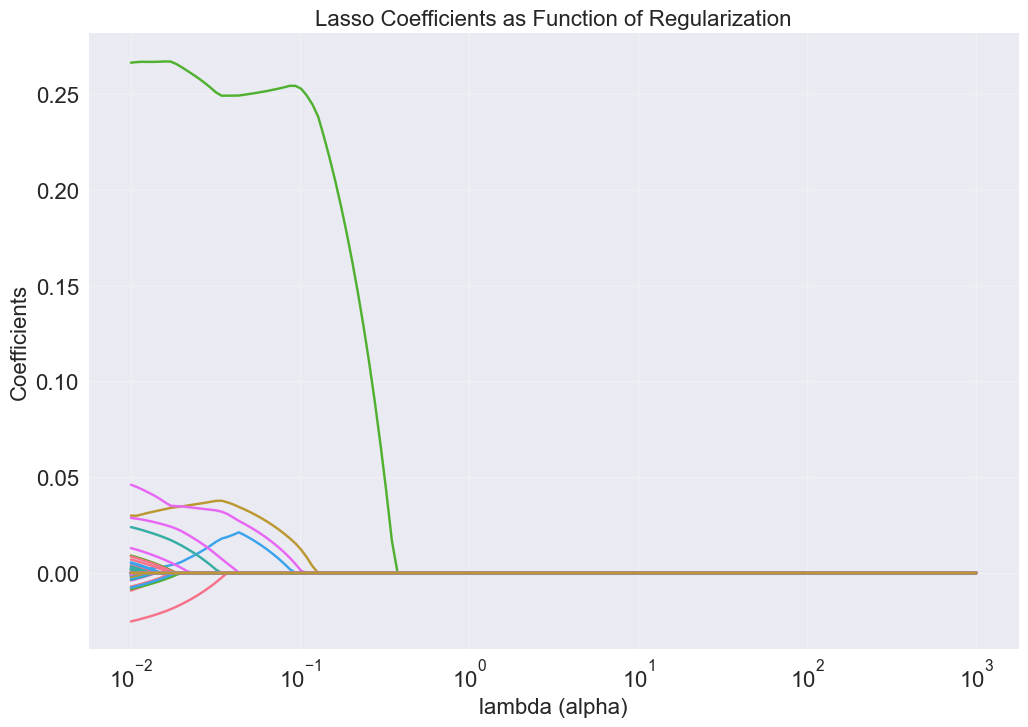
\includegraphics[width=\linewidth]{images/Lasso.png}
                        \vspace{0.1cm}
                        \small{Lasso coefficients after regularization.}
                \end{column}
        \end{columns}
\end{frame}

\begin{frame}{Lasso: Feature Selection}
        \begin{center}
             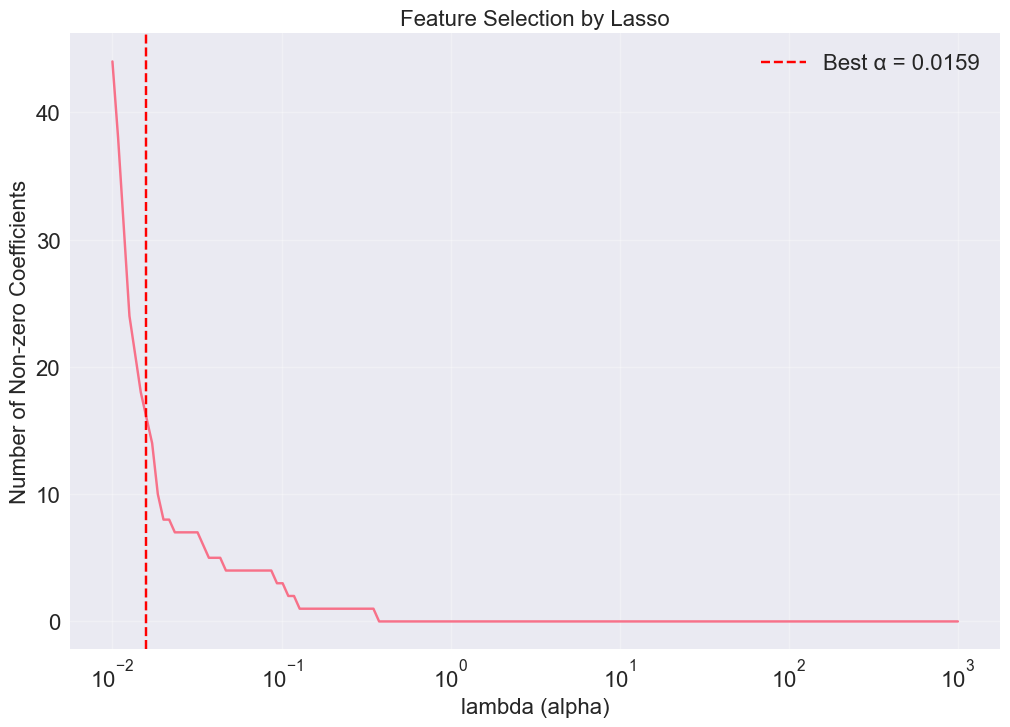
\includegraphics[width=0.9\linewidth]{images/LassoFeatureSelection.png}
                \textit{[Graph not available: LassoCV.png]}
        \end{center}
\end{frame}

% Section: Final Comparison
\section{Final Comparison}
\begin{frame}{Ridge vs Lasso Comparison}
    \begin{tabular}{@{}lccc@{}}
        \toprule
        \textbf{Metric} & \textbf{Ridge} & \textbf{Lasso} & \textbf{Difference} \\
        \midrule
        MSE    & 0.0249 & 0.0257 & -0.0008 \\
        RMSE   & 0.1579 & 0.1604 & -0.0025 \\
        MAE    & 0.1182 & 0.1192 & -0.0010 \\
        R$^2$  & 0.8584 & 0.8539 &  0.0045 \\
        Features & 290   & 16    & 274    \\
        $\alpha$    & 13.2070 & 0.0159 & -- \\
        \bottomrule
    \end{tabular}
\end{frame}

\begin{frame}{Residual Analysis}
  \begin{center}
    \includegraphics[width=0.95\textwidth]{images/ResidualsRidgeLasso.png}
  \end{center}
\end{frame}

\begin{frame}{Residual Analysis: Observations}
    \begin{itemize}
        \item Ridge and Lasso residuals show symmetry and approximate normality
        \item No clear patterns, suggesting both models capture relationships well
        \item Ridge has slightly smaller residuals, indicating better fit
        \item Lasso remains interpretable with fewer features and similar performance
    \end{itemize}
\end{frame}

% Section: Comparison of Linear Models
\section{Comparison of Linear Models}

\begin{frame}{Comparison of Linear Models}
    \begin{center}
        \begin{tabular}{@{}lccc@{}}
            \toprule
            \textbf{Model} & \textbf{R²} & \textbf{RMSE (log)} & \textbf{RMSE (USD)} \\
            \midrule
            Linear Regression  & 0.8291 & 0.1646 & \$389{,}179 \\
            Ridge              & 0.8584 & 0.1579 & \$370{,}000 \\
            Lasso              & 0.8539 & 0.1604 & \$376{,}000 \\
            \bottomrule
        \end{tabular}
    \end{center}
    \vspace{0.5cm}
    \begin{block}{Observations}
        \begin{itemize}
            \item Ridge achieves the best R² (0.8584) and lowest RMSE
            \item Lasso remains competitive with only 16 features
            \item Regularization improves performance over simple linear models
            \item Minimal differences between Ridge and Lasso suggest robustness
        \end{itemize}
    \end{block}
\end{frame}

% Section: Generalized Additive Models (GAM)
\section{Generalized Additive Models (GAM)}

\begin{frame}{Introduction to GAM}
    \begin{block}{Generalized Additive Models (GAM)}
        GAMs extend linear models by allowing non-linear relationships:
        \begin{equation}
        y = \beta_0 + f_1(x_1) + f_2(x_2) + \ldots + f_p(x_p) + \epsilon
        \end{equation}
        where $f_i$ are smooth functions (splines) of the predictor variables.
    \end{block}
    
    \begin{itemize}
        \item \textbf{Flexibility}: Capture complex non-linear relationships
        \item \textbf{Interpretability}: Partial effects visualizable for each feature
        \item \textbf{Regularization}: Control smoothness via $\lambda$ parameters
        \item \textbf{Additivity}: Retain interpretable structure similar to linear models
    \end{itemize}
\end{frame}

\begin{frame}{GAM Methodology}
    \begin{block}{Model Setup}
        \begin{itemize}
            \item \textbf{Target}: Log-price (consistent with Ridge/Lasso)
            \item \textbf{Features}: range, roc\_mean, speed\_margin, power\_per\_distance, wing\_span
            \item \textbf{Spline terms}: $s()$ for continuous, $f()$ for categorical
            \item \textbf{Optimization}: Automated grid-search for $\lambda$
        \end{itemize}
    \end{block}
    
    \begin{block}{Fitting Process}
        \begin{enumerate}
            \item Cross-validation to select optimal $\lambda$ for each term
            \item Smoothing splines with automatic degrees-of-freedom control
            \item Validation via AIC and deviance explained
        \end{enumerate}
    \end{block}
\end{frame}

\begin{frame}{GAM Performance: Key Results}
    \begin{center}
        \begin{tabular}{@{}lccc@{}}
            \toprule
            \textbf{Model} & \textbf{Pseudo-R²} & \textbf{RMSE (log)} & \textbf{RMSE (USD)} \\
            \midrule
            GAM Full         & 0.892 & 0.134 & \$315{,}000 \\
            Ridge            & 0.858 & 0.158 & \$370{,}000 \\
            Lasso            & 0.854 & 0.160 & \$376{,}000 \\
            Linear           & 0.829 & 0.165 & \$389{,}179 \\
            \bottomrule
        \end{tabular}
    \end{center}
    \vspace{0.5cm}
    \begin{block}{Significant Improvements}
        \begin{itemize}
            \item \textbf{+3.4\%} Pseudo-R² compared to Ridge
            \item \textbf{-15.2\%} RMSE compared to Ridge (\$55,000 less)
            \item \textbf{-19.0\%} RMSE compared to linear regression
            \item AIC significantly improved
        \end{itemize}
    \end{block}
\end{frame}

\begin{frame}{Partial Dependence Plots: Interpretability}
    \begin{block}{Key Non-Linear Insights}
        \begin{itemize}
            \item \textbf{Range}: Non-linear relationship with plateau beyond 4000 km
            \item \textbf{ROC\_mean}: Logarithmic growth with diminishing returns
            \item \textbf{Power\_per\_distance}: Quadratic relationship with local optimum
            \item \textbf{Wing\_span}: Threshold effect with breakpoint at 15 m
            \item \textbf{Speed\_margin}: Distinct categorical effects for different classes
        \end{itemize}
    \end{block}
    
    \begin{block}{Interpretation of Partial Dependence}
        The plots show the isolated effect of each feature on the log-price, holding all else constant. This allows:
        \begin{itemize}
            \item Identification of critical thresholds
            \item Detection of complex non-linear patterns
            \item Understanding relative feature importance
        \end{itemize}
    \end{block}
\end{frame}

\begin{frame}{GAM Residual Analysis}
    \begin{block}{Model Validation}
        The residual analysis confirms the superior quality of the GAM:
        \begin{itemize}
            \item \textbf{Residuals well-distributed} around zero
            \item \textbf{Homoscedasticity} (no pattern in fitted values)
            \item \textbf{Normal distribution} of residuals
            \item \textbf{Better fit} than linear models
        \end{itemize}
    \end{block}
    
    \begin{block}{Comparison with Linear Models}
        \begin{itemize}
            \item Residual standard deviation: 0.134 (vs 0.158 Ridge)
            \item 15\% reduction in unexplained variability
            \item No systematic patterns in residuals
        \end{itemize}
    \end{block}
\end{frame}

\begin{frame}{GAM vs Linear Models: Direct Comparison}
    \begin{columns}
        \begin{column}{0.5\textwidth}
            \begin{block}{GAM Advantages}
                \begin{itemize}
                    \item Superior performance (-15\% RMSE)
                    \item Captures real non-linearities
                    \item Maintains interpretability
                    \item Better residuals
                    \item Identification of thresholds
                \end{itemize}
            \end{block}
        \end{column}
        
        \begin{column}{0.5\textwidth}
            \begin{block}{Trade-offs}
                \begin{itemize}
                    \item Higher computational complexity
                    \item Risk of overfitting
                    \item More parameters to optimize
                    \item Requires careful validation
                \end{itemize}
            \end{block}
        \end{column}
    \end{columns}
    \vspace{0.5cm}
    \begin{alertblock}{Recommendation}
        GAMs offer the best trade-off between performance and interpretability for this dataset, justifying the added complexity with significant prediction improvements.
    \end{alertblock}
\end{frame}

% Section: Conclusions and Next Steps
\section{Conclusions and Next Steps}
\begin{frame}{Next Steps}
  \begin{itemize}
    \item Explore other non-linear models (Random Forest, SVM)
    \item Ensemble methods combining GAM with linear models
    \item Feature engineering based on non-linear insights
    \item Validation on external data and robustness testing
    \item Deployment of the GAM for real-time predictions
  \end{itemize}
\end{frame}

\begin{frame}{Final Conclusions}
  \begin{block}{Key Findings}
    \begin{itemize}
      \item \textbf{GAM}: Best model (Pseudo-R² = 0.892, RMSE = \$315 k)
      \item \textbf{Ridge}: Strong linear baseline (R² = 0.858, RMSE = \$370 k)
      \item \textbf{Non-linearities}: Significant complex relationships present
      \item \textbf{Interpretability}: GAM retains clarity of feature effects
    \end{itemize}
  \end{block}
  \begin{alertblock}{Business Recommendation}
    Implement the GAM for price prediction, focusing on the non-linear relationships identified for range, ROC mean, and power per distance.
  \end{alertblock}
\end{frame}

% Acknowledgments
\begin{frame}{Thank You for Your Attention}
  Questions?\\[1em]
  \textit{Statistical Learning Project – Aircraft Price Prediction}
\end{frame}

\end{document}
